\documentclass[11pt]{article}
\usepackage{geometry}                % See geometry.pdf to learn the layout options. There are lots.
\geometry{letterpaper}                   % ... or a4paper or a5paper or ... 
%\geometry{landscape}                % Activate for for rotated page geometry
\usepackage[parfill]{parskip}    % Activate to begin paragraphs with an empty line rather than an indent
\usepackage{daves,fancyhdr,natbib,graphicx,dcolumn,amsmath,lastpage,url}
\usepackage{amsmath,amssymb,epstopdf,longtable}
\usepackage{paralist}  % need to properly formulate standard answer blocks
\usepackage[final]{pdfpages}
\DeclareGraphicsRule{.tif}{png}{.png}{`convert #1 `dirname #1`/`basename #1 .tif`.png}
\pagestyle{fancy}
\lhead{CE 3372 Water Systems Design; Exam 1}
\rhead{Name:\_\_\_\_\_\_\_\_\_\_\_\_\_\_\_\_\_\_\_\_\_\_\_\_\_\_\_\_\_\_\_\_\_\_}
\lfoot{FALL 2017 A::}
\cfoot{}
\rfoot{Page \thepage\ of \pageref{LastPage}}
\renewcommand\headrulewidth{0pt}
\newcommand\tab[1][1cm]{\hspace*{#1}}



\begin{document}
%%%%%%%%%%%%%%%%%%%%%%%%%%%%%%%%%%%
\begingroup
\begin{center}
{\textbf{{ CE 3372 Water Systems Design Exam 1 }\\{Fall 2017}} }
\end{center}
\endgroup
Instructions:
\begin{enumerate}
\item Write your name on each sheet.
\item Read the entire exam before you begin -- use this initial scan to determine how to allocate your time on the exam.
\item Answer each problem -- if the problem is multiple choice \textbf{circle} the answer you think is correct.
\item For questions that ask you to identify items on a graphic, make your markings obvious and distinctive.  Use labels as necessary to guide the reader to your answer.
\item For questions that require analysis and calculations, show your work for full credit -- an answer alone, whether or not correct is insufficient demonstration of ability to solve the problem.
\item If you need to make an assumption, clearly state the assumption to receive partial credit.
\item If you do work on additional sheets, hand in those sheets with this exam, and put your name on each additional sheet.
\item If you delete an answer, clearly circle the entire deleted portion, then draw a diagonal line through the deleted portion, and write the word \textbf{delete} next to the diagonal line.
\end{enumerate}
%%%%%%%%%%%%%%%%%%%%%%%%%%%
Useful Equations and Material Properties: \\~\\
\begin{tabular}{p{2in} p{4in} p{0.5in}}
Hazen-Williams (SI) & $Q = 0.849~A~C_h~R^{0.63}~S^{0.54}$ & (1) \\
~&~&~\\
Reynolds number & ${Re}=\frac{VD}{\nu}$ & (2) \\
~&~&~\\
Friction factor (Jain) & $f = \frac{0.25}{[log(\frac{k_s}{3.7D} + \frac{5.74}{Re^{0.9}})]^2} $ & (3) \\
~&~&~\\
Darcy-Weisbach Loss Model & $h_{loss}=f\frac{L}{D}\frac{V^2}{2g} = \frac{8fLQ^2}{\pi^2gD^5} $& (4) \\
~&~&~\\
Discharge (Jain) & $ Q=-2.22D^{5/2} \times \sqrt{gh_f/L}\times[log_{10} (\frac{k_s}{3.7D} + \frac{1.78\nu}{D^{3/2}\sqrt{gh_f/L}} )] $ & (5) \\
~&~&~\\
NPSH Available & $NPSH_A = H_{abs.} + H_s -H_f - H_{vp} $& (6) \\
~&~&~\\
Vapor Pressure ($H_2O$)@25C & 3.170 $kPa$ & (7) \\
~&~&~\\
P$_{abs.}$@1000 meters & 87.586 $kPa$ & (8) \\
~ & ~ & ~ \\
Sp. Weight ($H_2O$)@25C & 9781 $N/m^3$ & (9) \\

\end{tabular}
\\








\clearpage
\begin{enumerate}
%\item ``Water for household needs: drinking, food preparation, personal hygiene, washing clothes and dishes, flushing toilets, and watering lawns and gardens'' describes which use category below?
%\begin{enumerate}[a)]
%\item Commercial Use
%\item Domestic Use
%\item Navigation (Inland) Use
%\item Irrigation Use
%\item Industrial Use
%\end{enumerate}

\item ``Application of water on lands to assist in growing of crops and pasture; maintain vegetative growth in recreational lands; maintain vegetative growth in ornamental displays'' describes which use category below?
\begin{enumerate}[a)]
\item Commercial Use
\item Domestic Use
\item Navigation (Inland) Use
\item Irrigation Use
\item Industrial Use
\end{enumerate}

\item ``Water for fabrication, processing, washing, and cooling in the production of manufactured items'' describes which use category below?
\begin{enumerate}[a)]
\item Commercial Use
\item Domestic Use
\item Navigation (Inland) Use
\item Irrigation Use
\item Industrial Use
\end{enumerate}

\item ``Water used as part of navigational systems to provide sufficient pool elevations for commercial waterborne cargo shipment'' describes which use category below?
\begin{enumerate}[a)]
\item Commercial Use
\item Domestic Use
\item Navigation (Inland) Use
\item Irrigation Use
\item Industrial Use
\end{enumerate}

\item The Los Angeles aqueduct system is best described as which kind of system?
\begin{enumerate}[(a)]
\item Water use system
\item Water control system
\item Environmental restoration system
\item Strategic withdrawl system
\end{enumerate}
\clearpage

\begin{figure}[h!] %  figure placement: here, top, bottom, or page
   \centering
   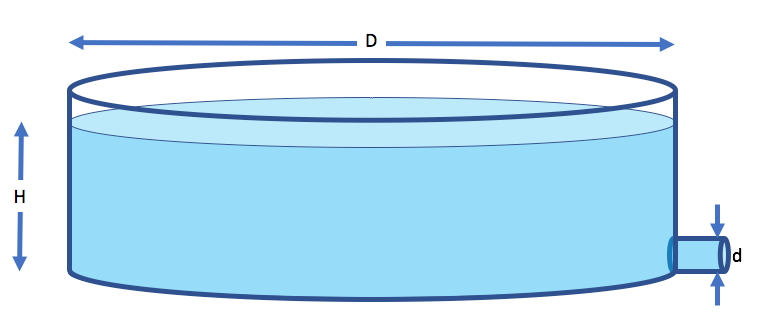
\includegraphics[width=4in]{Tank.jpg} 
   \caption{Circular Tank}
   \label{fig:Tank}
\end{figure}
\item Figure \ref{fig:Tank} is a circular (plan view) detention pond. 
The tank diameter, $D$, is 30 meters. 
The outlet diameter, $d$, is 127 millimeters.   
The initial depth in the pond is 2 meters.
Assume the discharge velocity is $V(t)=\sqrt{2gH(t)}$
\begin{enumerate}[(I)]
\item What is the outflow rate in Liters-per-second, if there is a supply of water that maintains the tank depth at 2 meters?
~\\~\\~\\
\item What is the time, in hours, for the tank to drain if there is no external supply and the discharge coefficient is unity ($c_d = 1$)?

\end{enumerate}


\clearpage
%%%%%%%%%%%%%%%%%%%%%%%%%%%%%%%%%%%%%%%%%%%%%%%%%
%%%%%%%%%%%PROBLEM 2 %%%%%%%%%%%%%%%%%%%%%%%%%%%%%%%
%%%%%%%%%%%%%%%%%%%%%%%%%%%%%%%%%%%%%%%%%%%%%%%%%
\item The questions below page refer to Figure \ref{fig:sewer} on the following page . 
\begin{enumerate}[(I)]
\item Is the design flow in the drawing from left-to-right, or right-to-left?
~\\
~\\
\item What object is depicted at station STA 54+05.00 in the plan view portion of the drawing?
~\\
~\\
\item The elevation view drawing depicts a drop at a junction box.  What is the bottom elevation of the junction box indicated on the drawing?
~\\
~\\
\item What is the diameter of the conduits indicated on the drawing?
~\\
~\\
\item What is the slope (in percent) of the storm sewer conduits?
~\\
~\\
\item Relative to the drop structure, what is the flow-line (invert) elevation of the left-most sewer pipe?
~\\
~\\
\item Relative to the drop structure, what is the flow-line (invert) elevation of the right-most sewer pipe?
~\\
~\\
\item Relative to the drop, structure what is the soffit (crown) elevation of the left-most sewer pipe?
~\\
~\\
\item Relative to the drop structure, what is the soffit (crown) elevation of the right-most sewer pipe?
~\\
~\\
\end{enumerate}
\begin{figure}[ht!] %  figure placement: here, top, bottom, or page
\centering
   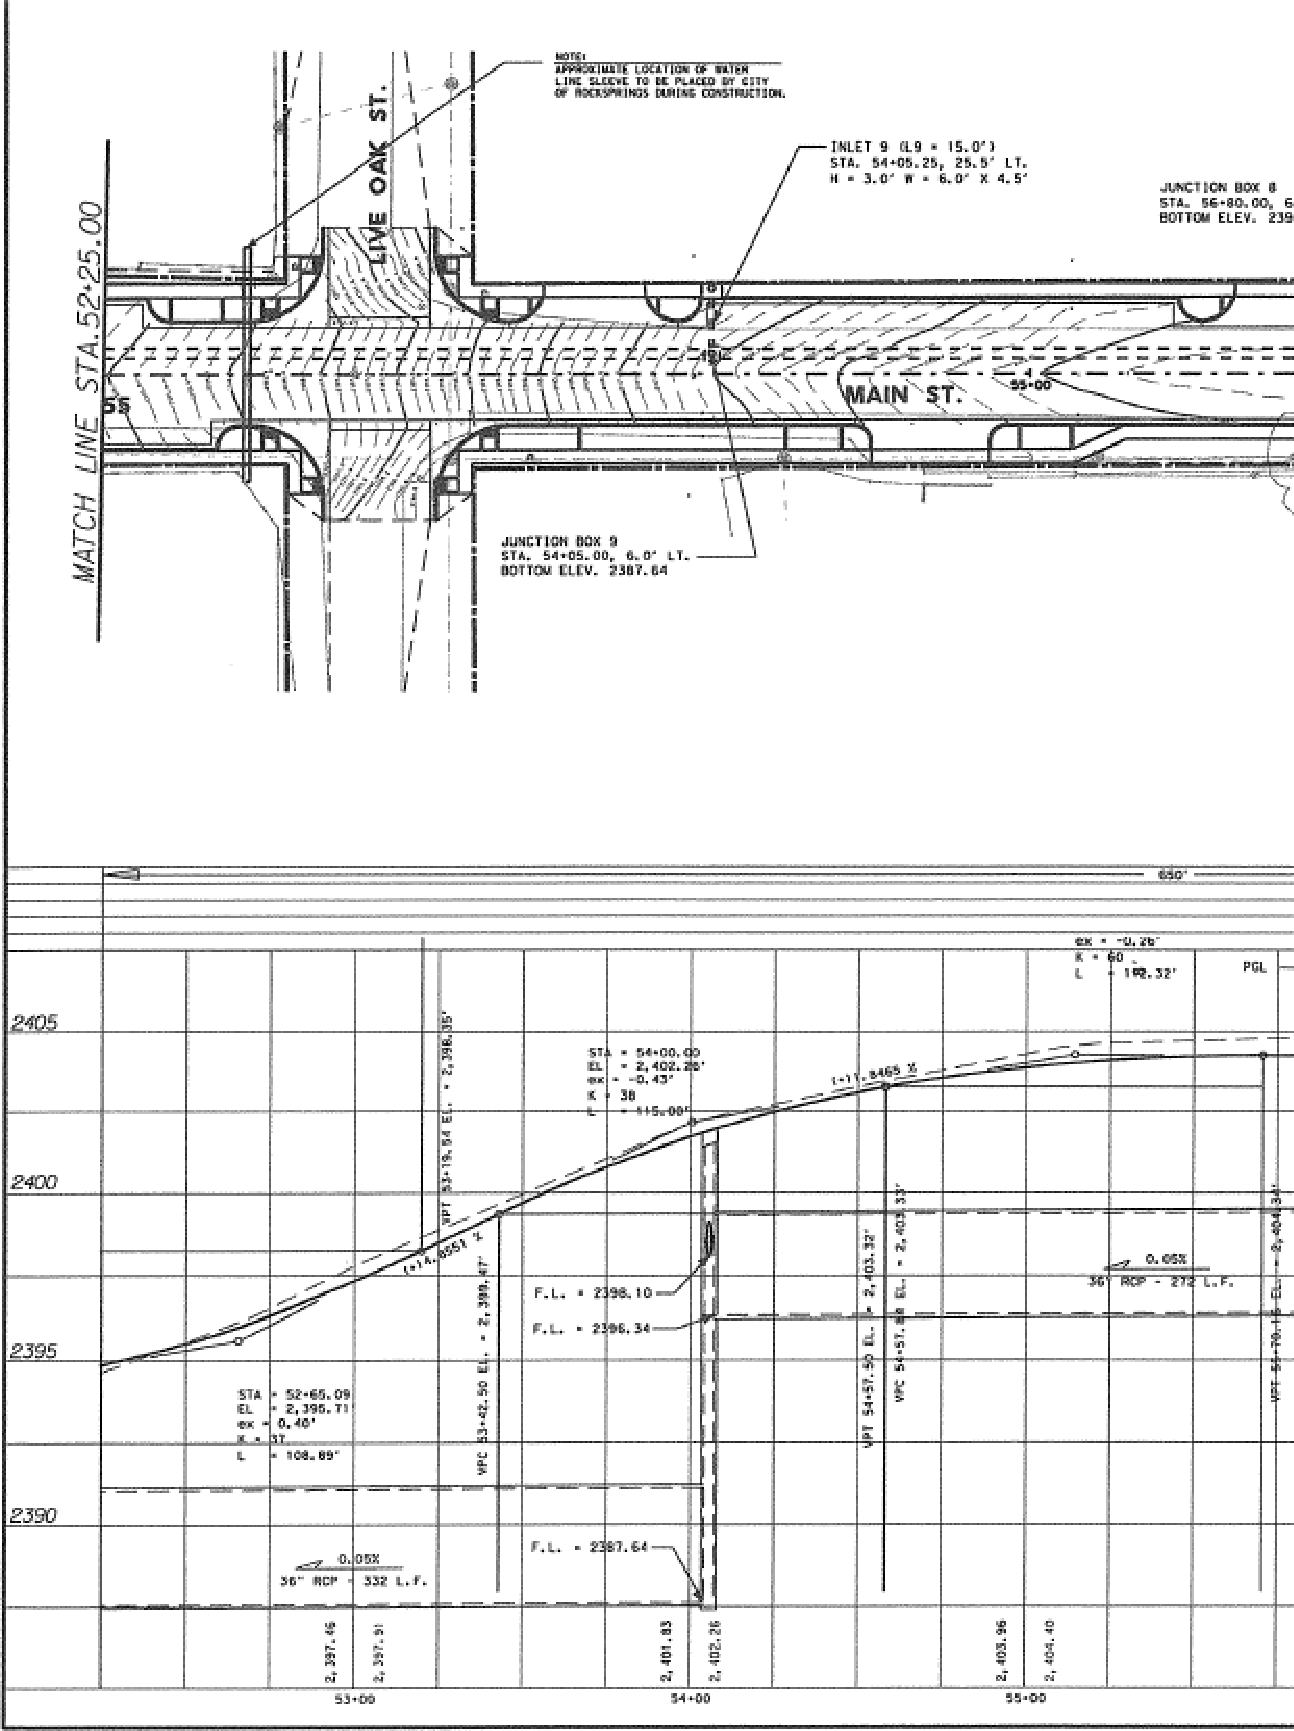
\includegraphics[width=6in]{sewer.pdf}
   \caption{Plan and profile of a storm sewer system}
   \label{fig:sewer} 
\end{figure}
\clearpage
%%%%%%%%%%%%%%%%%%
%%%%%%%%%%%%%%%%%%
% Africa Pipelines YOYO              %
%%%%%%%%%%%%%%%%%%
\item Figure \ref{fig:AfricaSystem} is an aerial image of a pipeline system with preliminary engineering sketches of the system (lower left panel) and a detail sketch of the terminal small storage tank (upper right panel). 
The 3,200 meter long pipeline lifts 25C water ($\rho = 997~kg/m^3$, $\nu = 8.94 \times 10^{-7}~m^2/s$) from a treatment plant on the downstream face of Gulameta Dam through a 127 millimeter high-density polyethylene (HDPE) pipe ($k_s = 0.0015~mm$) to a large diameter at-grade cylindrical storage tank.
A secondary, 800 meter long pipeline carries water from the large diameter storage tank to a small, cylindrical ($D = 1~meter$), elevated storage tank at the village school.   Both storage tanks have float valves to prevent overflow and maintain the indicated water pool elevations. 

\begin{figure}[htbp] %  figure placement: here, top, bottom, or page
   \centering
   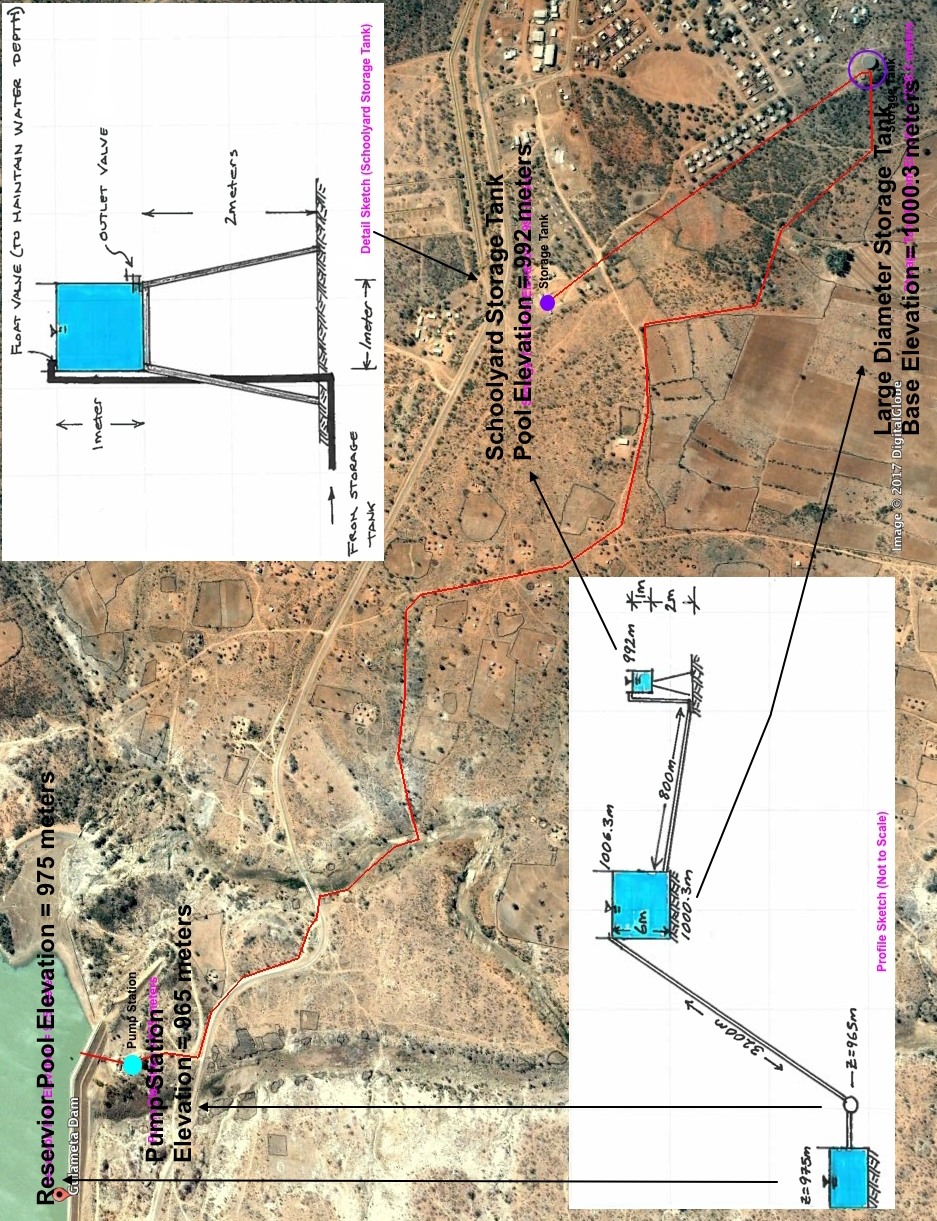
\includegraphics[width=6in]{AfricaSystem.jpg} 
   \caption{Water Supply System in Re-Developing Nation}
   \label{fig:AfricaSystem}
\end{figure}

\begin{enumerate}[(I)]
\item What is the pool elevation, in meters, of the supply reservoir (Lake Gulameta)? 
\begin{enumerate}[a)]
\item 965 meters
\item 975 meters
\item 3165.2 feet
\item 3198 feet
\end{enumerate}
\item What is the pump centerline elevation, in meters, that supplies water to the HDPE pipeline?
\begin{enumerate}[a)]
\item 965 meters
\item 975 meters
\item 3165.2 feet
\item 3198 feet
\end{enumerate}
\item What is the length of HDPE pipeline, in meters, from the pump station to the large diameter storage tank?
\begin{enumerate}[a)]
\item 800 meters
\item 3200 meters
\item 2624 feet
\item 10,496 feet
\end{enumerate}
\item What is the pool elevation, in meters, in the large diameter storage tank, assuming the float valve is correctly operating?
\begin{enumerate}[a)]
\item 1000.3 meters
\item 1000.6 meters
\item 1003.6 meters
\item 1006.3 meters
\end{enumerate}
\item What is the length of HDPE pipeline, in meters, from the large diameter storage tank to the schoolyard storage tank?
\begin{enumerate}[a)]
\item 800 meters
\item 3200 meters
\item 2624 feet
\item 10,496 feet
\end{enumerate}
\item What is the pool elevation, in meters, in the schoolyard storage tank, assuming the float valve is correctly operating?
\begin{enumerate}[a)]
\item 989 meters
\item 990 meters
\item 991 meters
\item 992 meters
\end{enumerate}
\item What is the ground surface elevation, in meters, at the schoolyard storage tank?
\begin{enumerate}[a)]
\item 989 meters
\item 990 meters
\item 991 meters
\item 992 meters
\end{enumerate}
\item Write the Modified Bernoulli (Energy) Equation for the portion of the system from the water supply reservoir (Lake Gulameta) to the large diameter storage tank. 
\clearpage
\item Write the Modified Bernoulli (Energy) Equation for the portion of the system from the large diameter storage tank to the schoolyard storage tank. \\
~\\~\\~\\~\\~\\~\\~\\~\\~\\~\\~\\~\\~\\~\\~\\~\\
\item Assume the float valve at the schoolyard fails in the open position, and the schoolyard tank overflows.  Using the Modified Bernoulli (Energy) Equation for the portion of the system from the large diameter storage tank to the schoolyard storage tank, and neglecting minor loss terms (but not the pipeline loss), determine the flow rate in the system in Liters-per-second.
\clearpage
\item Using the flow rate just computed, and the Modified Bernoulli (Energy) Equation for the portion of the system from from the water supply reservoir (Lake Gulameta) to the large diameter storage tank, and neglecting minor loss terms (but not the pipeline loss), determine the required pump head (added head).
~\\~\\~\\~\\~\\~\\~\\~\\~\\~\\~\\~\\~\\~\\~\\~\\~\\~\\~\\~\\~\\~\\~\\~\\
\item Assume the float valve at the schoolyard is operating normally, but someone accidentally leaves the outlet valve (nominal diameter = 75 mm) from the tank open.  Estimate the required flow rate in the system in Liters-per-second to sustain the indicated pool elevations.
\clearpage
\item Figure \ref{fig:pumps} is a set of pump curves for a pump at different impeller speeds.  Circle the portion of the graphic that contains information about the Net Positive Suction Head (NPSH) required by the pump.
\item Assuming the schoolyard overflow condition is the most flow the pump will have to deliver, select a pump speed from one of the five on Figure \ref{fig:pumps} below.  Indicate which curve you selected, show the operating point.  Indicate if you need two pumps in series to supply the necessary head.
\item Estimate the NPSH required for the pump at your operating point.

\begin{figure}[h]
\centering
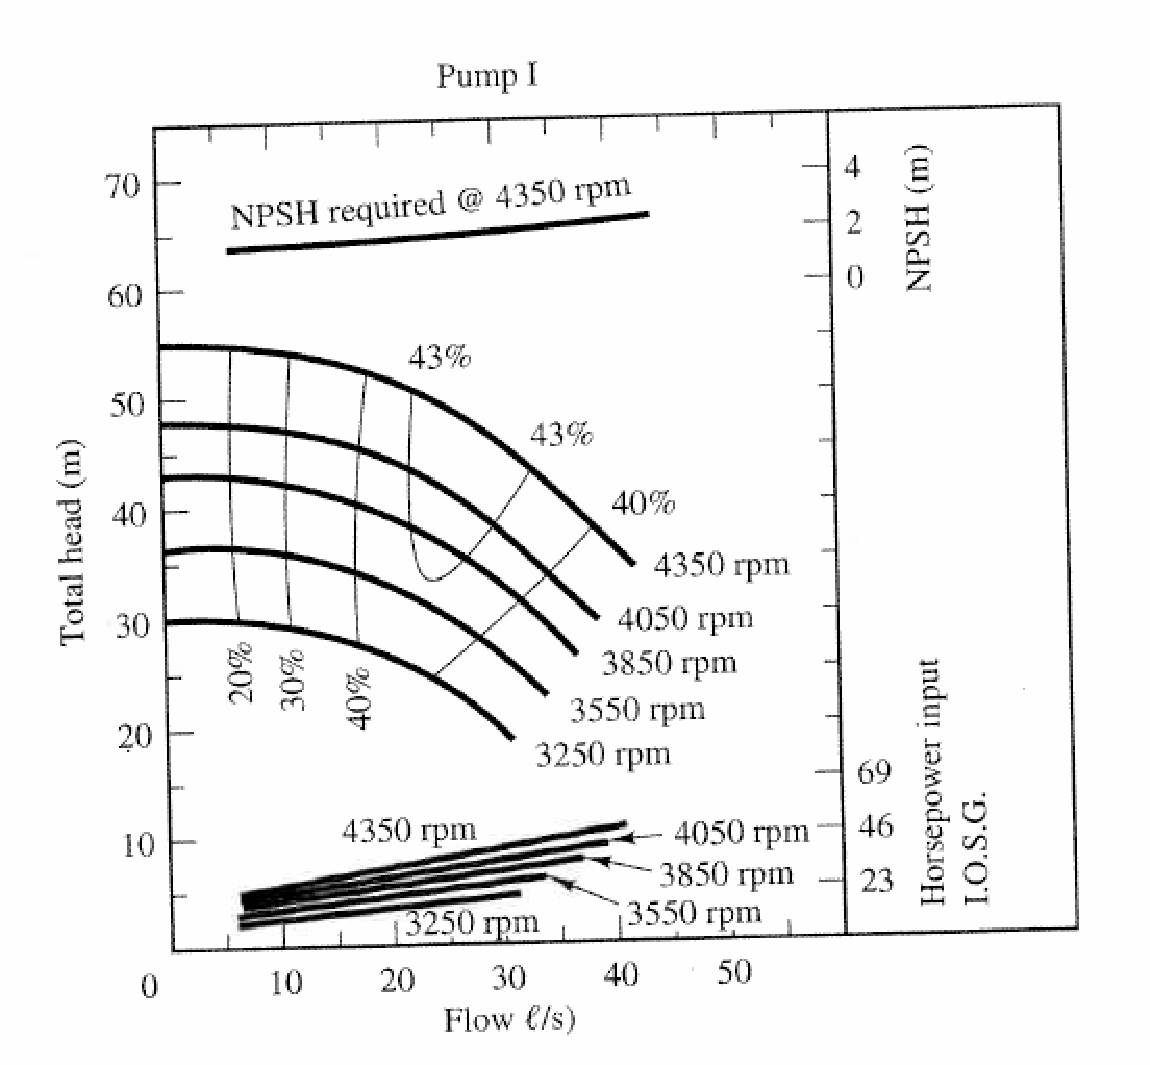
\includegraphics[width=0.7\textwidth]{pump1.pdf}%
%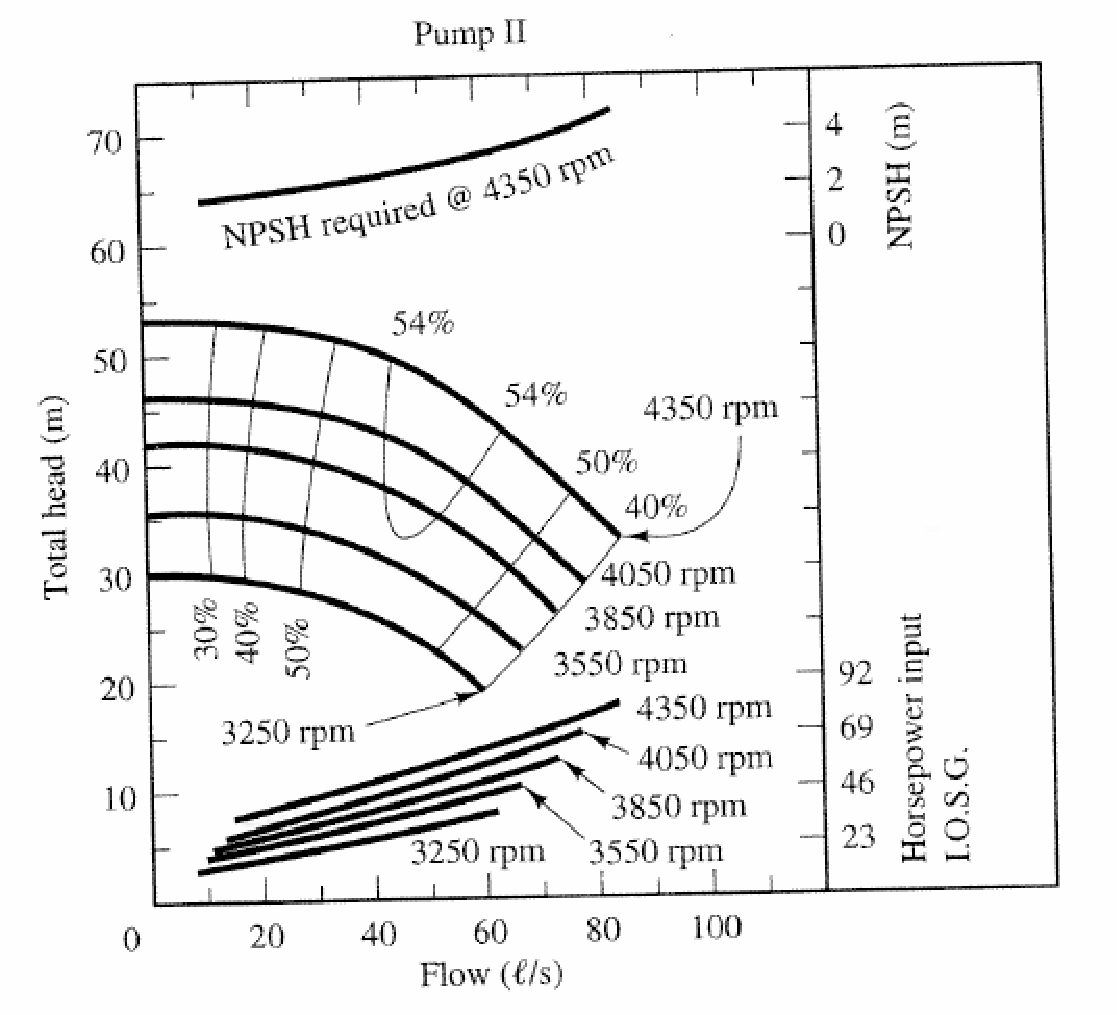
\includegraphics[width=0.5\textwidth]{pump2.pdf}\\%[0.5cm]%can add fill space here if you want
%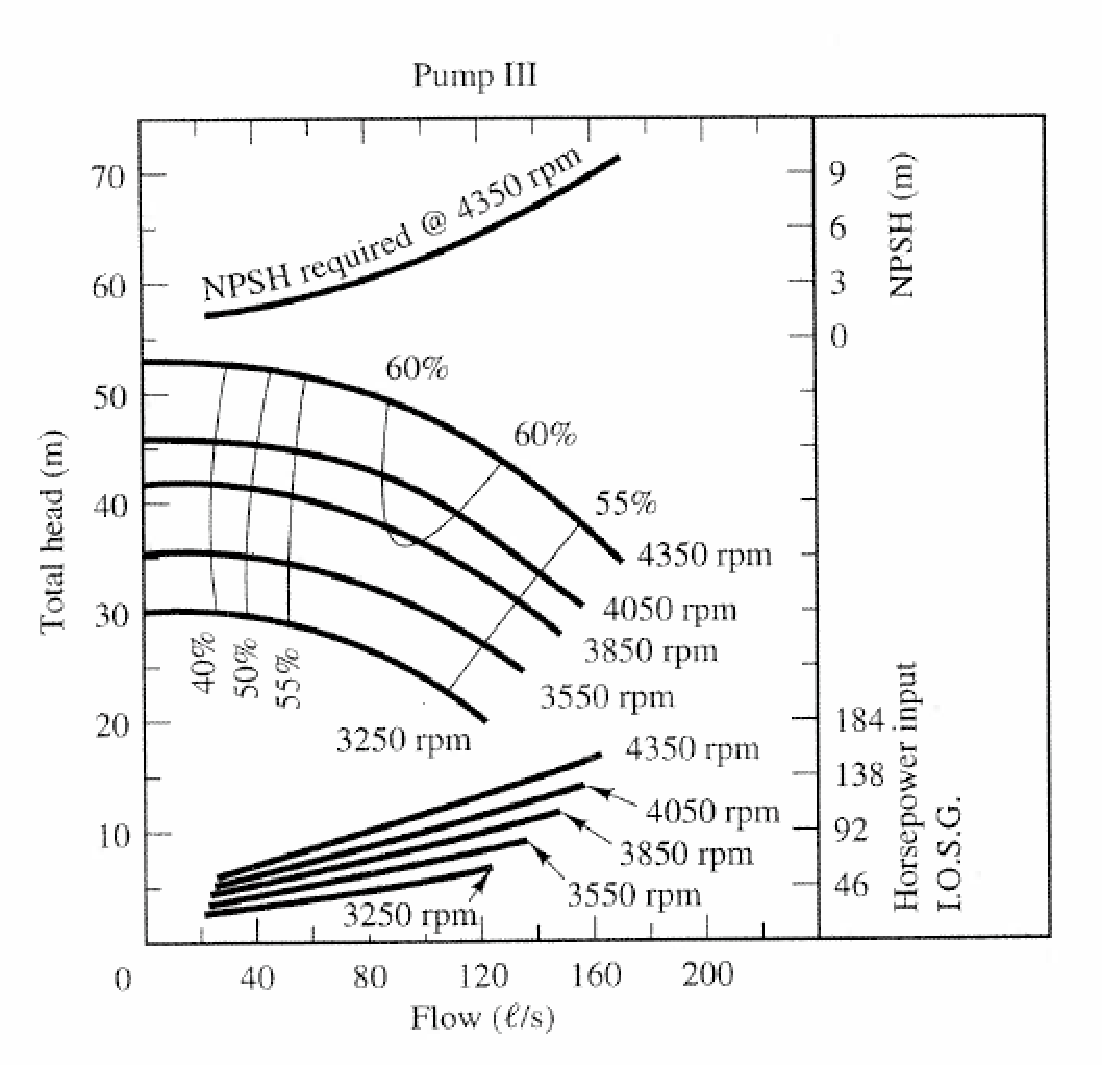
\includegraphics[width=0.5\textwidth]{pump3.pdf}%
%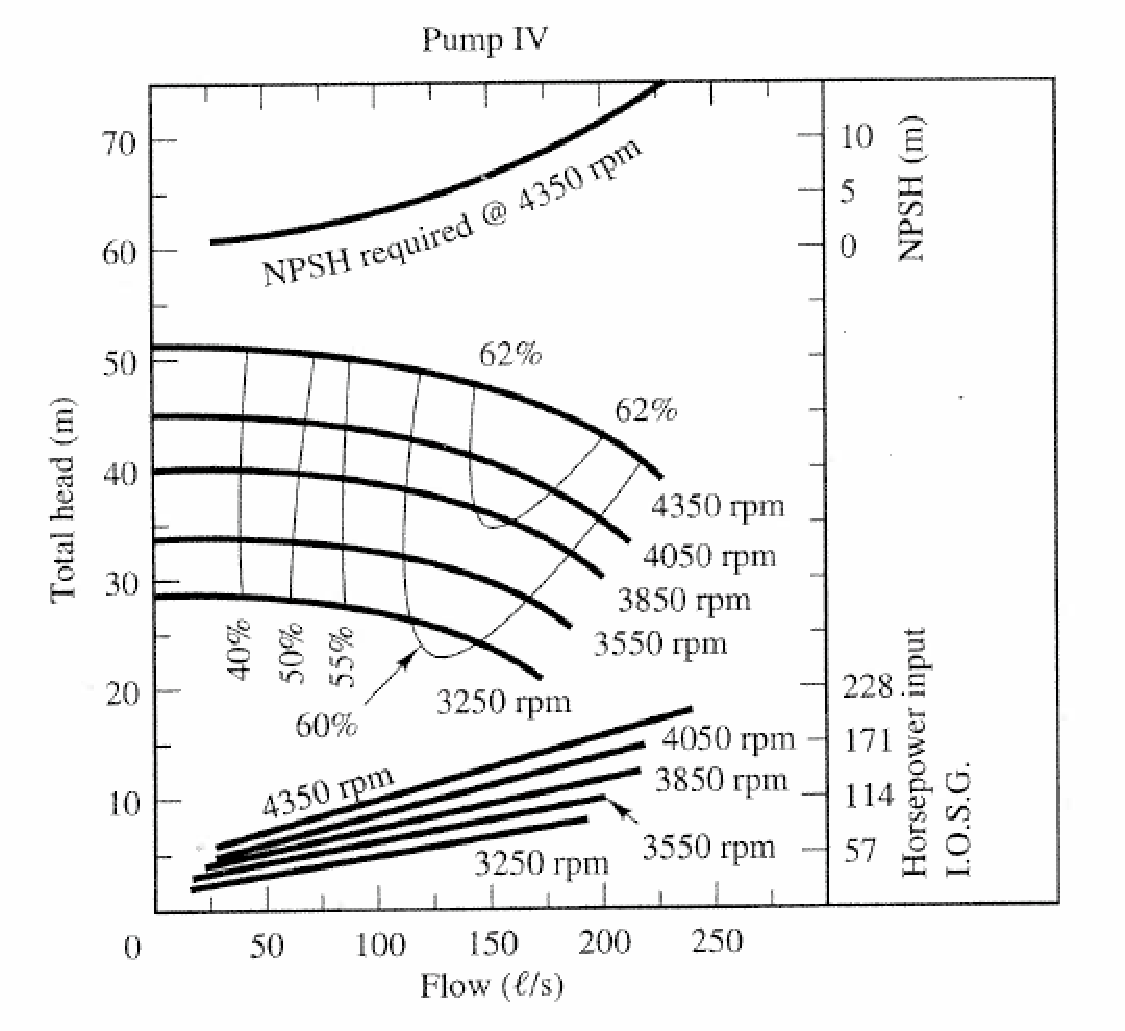
\includegraphics[width=0.5\textwidth]{pump4.pdf}%
\caption{Pump curves for 5 different impeller speeds.}
\label{fig:pumps}
\end{figure}
\item Estimate the NPSH available for the system, you can neglect inlet piping and minor losses.  Assume the water is at 25 degrees Celsius.
~\\~\\~\\
\item Is there sufficient NPSH available for the system to function at the design flow rate without cavitation?
\end{enumerate}

\clearpage
%%%%%%%%%%%%%%%%%%%%%%%%%%%%%%%
%%%%%%% END AFRICA PROBLEM %%%%%%%%%%%
%%%%%%%%%%%%%%%%%%%%%%%%%%%%%%%

\item Figure \ref{fig:wheatstone_bridge} is a pipe network with the following properties:
\begin{figure}[h!] %  figure placement: here, top, bottom, or page
\centering
   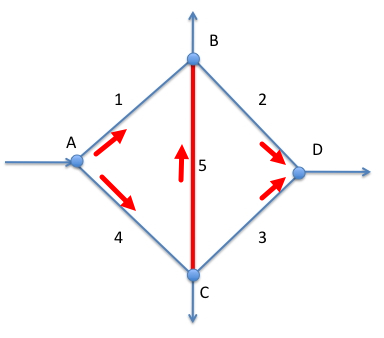
\includegraphics[width=3.1in]{wheatstone_bridge.jpg}
   \caption{Pipe network}
   \label{fig:wheatstone_bridge} 
\end{figure}

\begin{table}[h!]
%\footnotesize
   \centering
   \caption{Network properties for Figure \ref{fig:wheatstone_bridge}}
\begin{tabular}{lll}
\hline
Node&Demand (lps)&  Elevation(m) \\
\hline
A & -0.60 & 0.00 \\
B &  0.15   & 0.00 \\
C & 0.15 & 0.00 \\
D & 0.30 & 0.00 \\
\hline
Pipe& Length (m)&  Diameter (mm)\\
\hline
1 & 10,000 & 77.0 \\
2 & 10,000 & 77.0 \\
3 & 10,000 & 77.0 \\
4 & 10,000 & 77.0 \\
5 & 14,000 & 77.0 \\
\end{tabular}
\label{tab:wheatstone1}
\normalsize
\end{table}


%%%%%%%%%%%%%%%%%%%%%%%%%%%%

Referring to Figure \ref{fig:wheatstone_bridge}, and Table \ref{tab:wheatstone1} the flow distribution is:
%standard answer set
\begin{enumerate}[(A)]
\item $[Q_1,~Q_2,~Q_3,~Q_4,~Q_5~]~=$[0.30,-0.15,-0.15,0.30,-0.60] LPS
\item $[Q_1,~Q_2,~Q_3,~Q_4,~Q_5~]~=$[0.30,0.15,0.15,0.30,0.30] LPS
\item $[Q_1,~Q_2,~Q_3,~Q_4,~Q_5~]~=$[0.30,0.15,0.15,0.00,0.50] LPS
\item $[Q_1,~Q_2,~Q_3,~Q_4,~Q_5~]~=$[0.30,0.15,0.15,0.30,0.00] LPS
\end{enumerate}
%\item Referring to Figure \ref{fig:wheatstone_bridge}, assuming the average friction factor is $0.033$, the head loss, in feet, from Node A to Node C is closest to
%%standard answer set
%\begin{enumerate}[(A)]
%\item 1.25 meters 
%\item 2.50 meters
%\item 5.00 meters
%\item 10.0 meters
%\end{enumerate}
%\item Referring to Figure \ref{fig:wheatstone_bridge}, if the demands at all nodes are those in Table \ref{tab:wheatstone1}, and pipe 2 is decreased to a diameter of 50.8 mm, the discharge in pipe 5 is closest to
%%standard answer set
%\begin{enumerate}[(A)]
%\item 0.00 lps, from Node C to Node B  %Correct
%\item 0.15 lps, from Node B to Node C
%\item 0.30 lps, from Node C to Node B
%\item 0.60 lps, from Node B to Node C
%\end{enumerate}
%\clearpage
%%%%%%%%%%%%%%%%%%%%%%%%%%%%
\end{enumerate}
\end{document}  
%%%%%%%%%%%%%%% Eeeee

%%%%%%%%%%%%%%%%%%%%%%%%%%%%%%%%%%%%%%%%%%%%%%%%%
%%%%%%%PROBLEM 1 %%%%%%%%%%%%%%%%%%%%%%%%%%%%%%%%%%%
%%%%%%%%%%%%%%%%%%%%%%%%%%%%%%%%%%%%%%%%%%%%%%%%%

\item A circular, 60-inch diameter, reinforced concrete sewer pipe ($n = 0.013$ )carries 50 MGD of wastewater to a lift station wet well.   Average slope along the flow path is 1.0\%.
%about 50 MGD%
\begin{enumerate} 
\item	Sketch the cross section, indicate the pipe diameter.
~\\
~\\
~\\
~\\
~\\
~\\
~\\
~\\
~\\
~\\
~\\
~\\
~\\
~\\
\item For the conditions in the problem statement, what is the flow rate in cubic feet per second?
~\\
~\\
\item What is the diameter of the pipe, in feet?
~\\
~\\


\item Use Manning's equation ($ Q = \frac{1.49}{n} A R^{(2/3)} S^{(1/2)} $) and determine the \textbf{pipe-full} discharge in cubic feet per second?
~\\
~\\
~\\
~\\
~\\
~\\
\clearpage
\item What is the pipe-full discharge ($Q_{f}$) in million gallons per day (MGD)?
~\\
~\\
~\\
\item Compute the ratio of actual flow ($\frac{Q}{Q_{f}}$) to full pipe flow.
~\\
~\\
~\\
\item What is the ratio of depth of actual flow to full flow ($\frac{d}{D}$) using the hydraulic element chart in Figure \ref{fig:hydraulic-elements}?  Use the highlighted curve.
~\\
~\\
~\\
\begin{figure}[ht!] %  figure placement: here, top, bottom, or page
\centering
   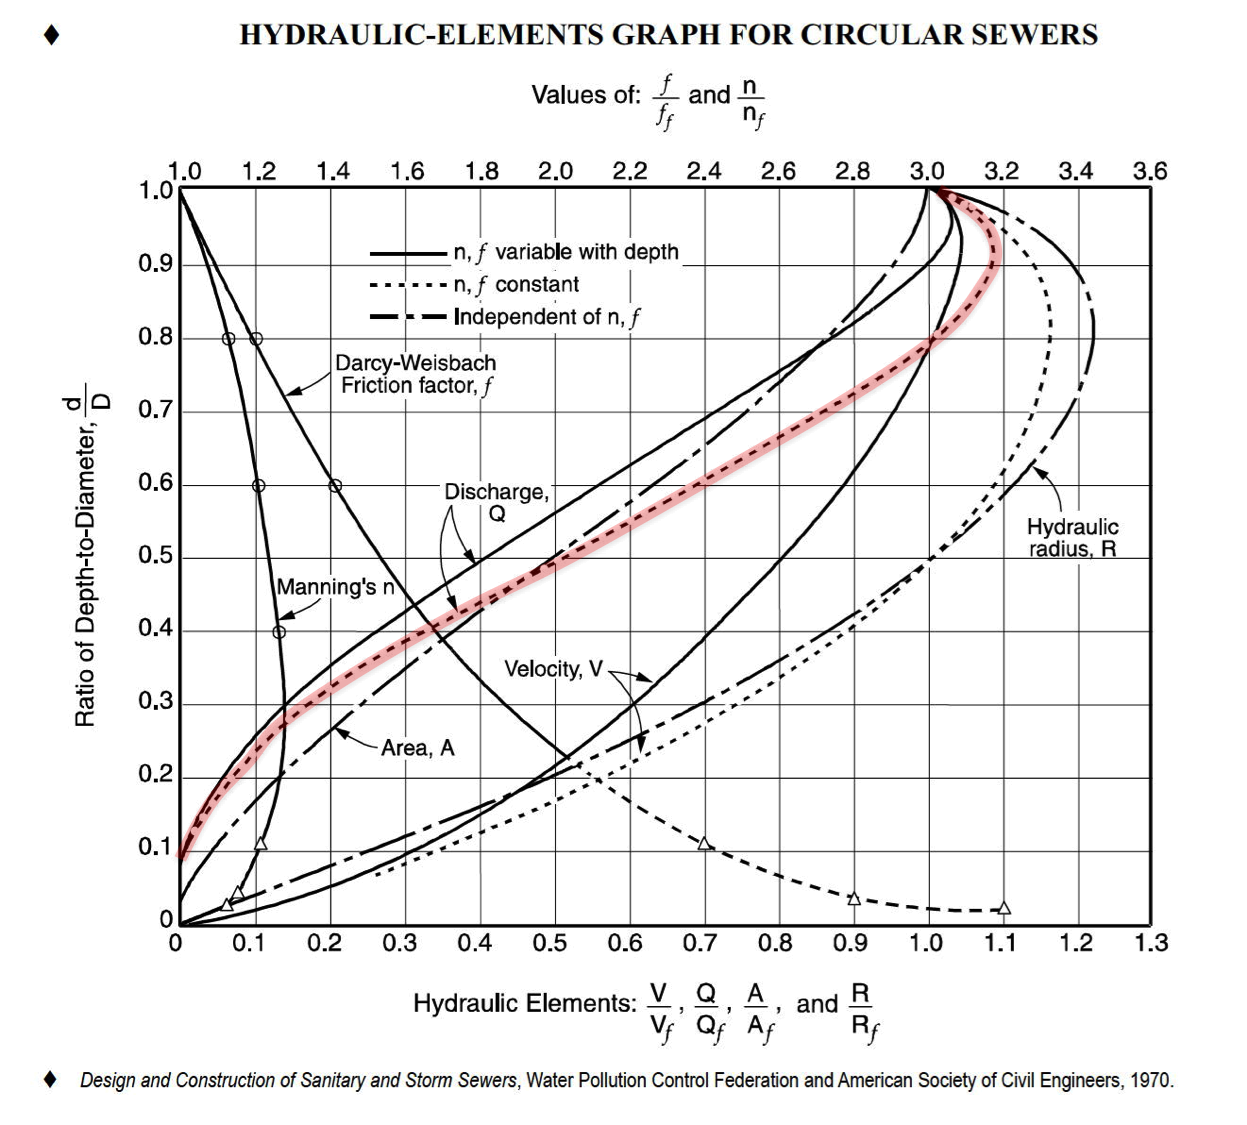
\includegraphics[width=4.5in]{hydraulic-elements.pdf}
   \caption{Hydraulic Elements Chart}
   \label{fig:hydraulic-elements} 
\end{figure}
\clearpage
\item What is the depth of actual flow in feet?
~\\
~\\
~\\
\item What is the depth of actual flow in inches?
~\\
~\\
~\\
\item Modify your sketch to include the water surface position and the approximate flow depth.
~\\
\item Is this portion of sewer close to surcharging?
~\\
\end{enumerate}

\clearpage
\item Figure \ref{fig:diameter-increase} is a plan-and profile of a portion of a storm sewer system.  Answer the questions on the following page.
\begin{figure}[ht!] %  figure placement: here, top, bottom, or page
\centering
   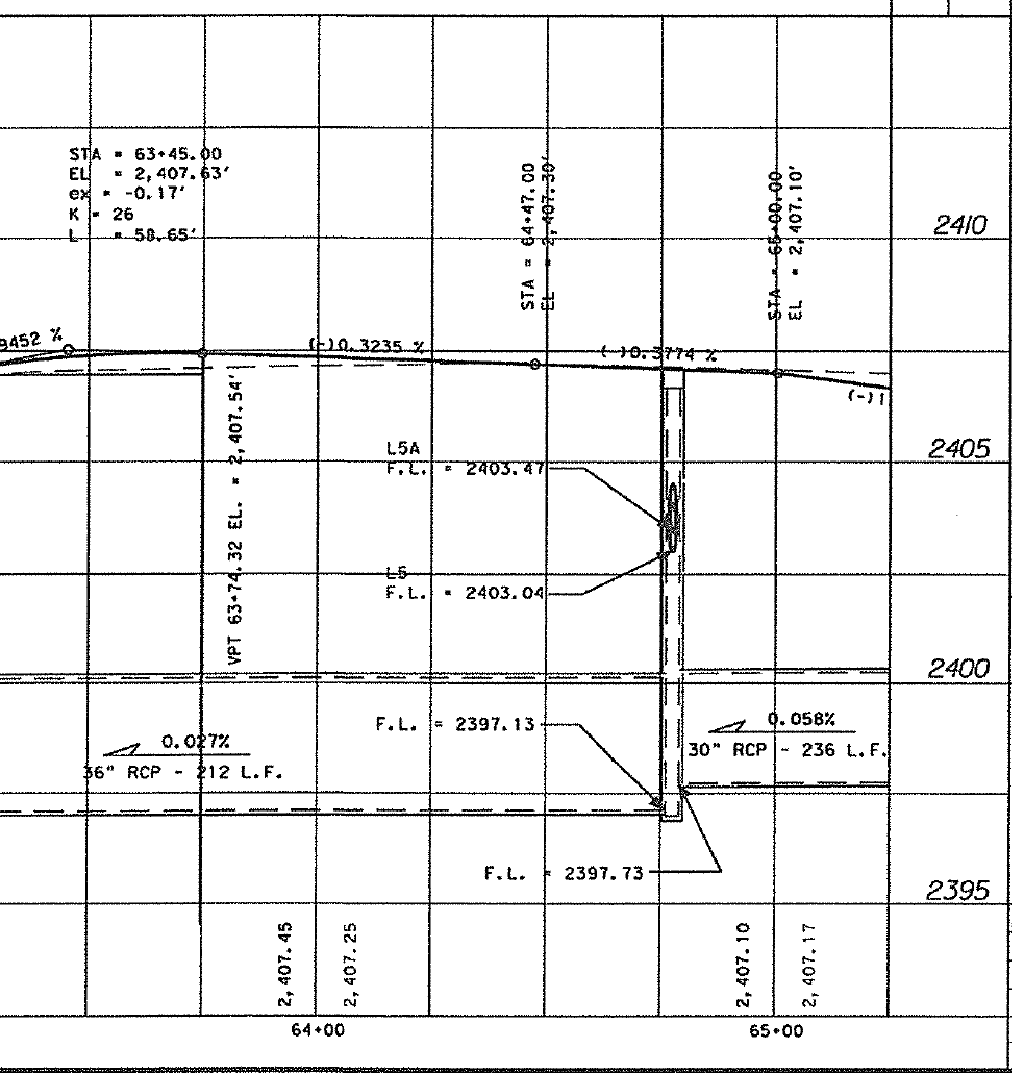
\includegraphics[width=5in]{diameter-increase.pdf}
   \caption{Plan and profile of a storm sewer system}
   \label{fig:diameter-increase} 
\end{figure}
\clearpage
\begin{enumerate}
\item What is the diameter of the conduit on the right-side of the drawing?
~\\
\item What is the slope of the conduit (in percent) on the right-side of the drawing?
~\\
\item What is the diameter of the conduit on the left-side of the drawing?
~\\
\item What is the slope of the conduit (in percent) on the right-side of the drawing?
~\\
\item What is the soffit (crown) elevation of the right-most sewer pipe?
~\\
\item What is the soffit (crown) elevation of the left-most sewer pipe?
~\\
\item What is the flow-line (invert) elevation of the right-most sewer pipe?
~\\
\item What is the flow-line (invert) elevation of the left-most sewer pipe?
~\\
\item Explain, using sketches as necessary, why sewer soffit elevations should match (or drop in the flow direction) at a junction when the pipe diameter increases moving downstream. 
\end{enumerate}

%%%%%%%%%%%%%%%%%%
% EPA-NET MSMD %%%%%%%%
%%%%%%%%%%%%%%%%%%
\item An EPA-NET simulation produced the  "full report" listed below.   
\begin{verbatim}
  **********************************************************************
  Link - Node Table:
  ----------------------------------------------------------------------
  Link           Start          End                Length  Diameter
  ID             Node           Node                   ft        in
  ----------------------------------------------------------------------
  1              2              3                    1000        12
  2              3              4                    1000        12
  3              2              5                    1000        12
  4              3              6                    1000        12
  5              5              6                    1000        12
  6              6              4                    1000        12
  7              1              2                    1000        12
  Node Results:
  ----------------------------------------------------------------------
  Node                Demand      Head  Pressure   Quality
  ID                     CFS        ft       psi          
  ----------------------------------------------------------------------
  2                     0.00     76.94     33.34      0.00
  3                     0.00     75.55     32.74      0.00
  4                     3.00     74.51     32.28      0.00
  5                     0.00     76.23     33.03      0.00
  6                     0.00     75.51     32.72      0.00
  1                    -3.00    100.00      0.00      0.00 Reservoir
  Link Results:
  ----------------------------------------------------------------------
  Link                  Flow  VelocityUnit Headloss    Status
  ID                     CFS       fps    ft/Kft
  ----------------------------------------------------------------------
  1                     1.76      2.25      1.39      Open
  2                     1.51      1.93      1.04      Open
  3                     1.24      1.57      0.71      Open
  4                     0.25      0.32      0.04      Open
  5                     1.24      1.57      0.71      Open
  6                     1.49      1.89      1.01      Open
  7                     3.00      3.82     23.06      Open
\end{verbatim}
\clearpage
Using the information contained in the EPA-NET report on the previous page:
\begin{enumerate}[a)]
\item How many pipes are in the network?
~\\
\item How many junctions (nodes) are in the network?
~\\
\item How many reservoirs/tanks are in the network?
~\\
\item Sketch the network, label the pipes, junctions, and reservoirs.   Indicate any demands at nodes.   Indicate the flow rates and flow directions on your sketch.
\end{enumerate}

\item  An EPA-NET simulation model for a reservoir-pump-network was constructed and operated for four (4) different operational scenarios.   Figure \ref{fig:epa-net-map} is a depiction of the network.   The numbers next to the nodes are Node\_ID values in the reports that follow, and the numbers next to the pipes are the Link\_ID values.  The network is supplied from a reservoir through a booster pump, both are depicted on Figure \ref{fig:epa-net-map}. 

\begin{figure}[h!] %  figure placement: here, top, bottom, or page
\centering
   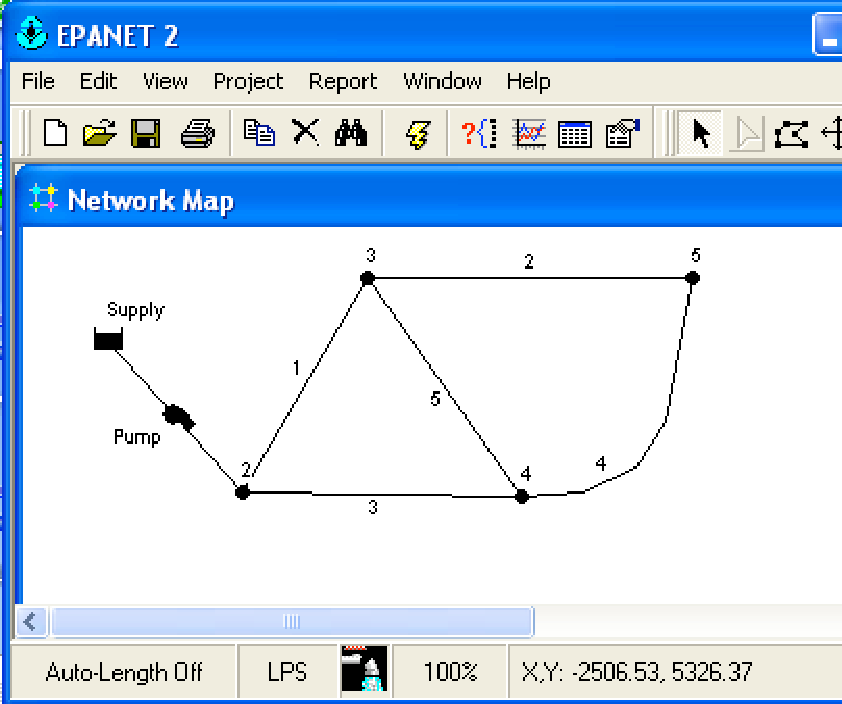
\includegraphics[width=3in]{epa-net-map.pdf}
   \caption{EPA-NET system topology.}
   \label{fig:epa-net-map} 
\end{figure}

Figure \ref{fig:epanet1} is the a portion of the summary report for simulation 1.   
Figure \ref{fig:epanet2} is the a portion of the summary report for simulation 2.  
Figure \ref{fig:epanet3} is the a portion of the summary report for simulation 3.  
Figure \ref{fig:epanet4} is the a portion of the summary report for simulation 4.

These four simulation represent different demand scenarios for the same system.



Interpret these reports, to answer the following questions:

\begin{enumerate}
\item Complete the table below.  $Q_{pump}$ is the discharge in liters-per-second through the pump station, $H_{Supply}$ is the head at the supply reservoir,  $H_{Node2}$ is the head at Node 2, and $\Delta H_{pump}$ is the added head supplied by the pump.
% Requires the booktabs if the memoir class is not being used
\begin{table}[htbp]
   \centering
      \caption{Pump Discharge and Supplied Head}
   \begin{tabular}{p{1in} p{1in} p{1in} p{1in} p{1in} } % Column formatting, @{} suppresses leading/trailing space
Simulation \# & $Q_{pump}$ & $H_{Supply}$ & $H_{Node2}$ & $\Delta H_{pump}$ \\
\hline
\hline
~~1 & ~ &~ & ~ & ~ \\
~ & ~ &~ & ~ & ~ \\
\hline
~~2 & ~ &~ & ~ & ~ \\
~ & ~ &~ & ~ & ~ \\
\hline
~~3 & ~ &~ & ~ & ~\\
~ & ~ &~ & ~ & ~ \\
\hline
~~4 & ~ &~ & ~ & ~ \\
~ & ~ &~ & ~ & ~ \\
\hline
   \end{tabular}
   \label{tab:pump-curve}
\end{table}

\item Complete the table below.  $Q_{pump}$ is the discharge in liters-per-second through the pump station, $\Delta H_{Node 2 -to- 5}$ is head loss in the system from Node 2 to Node 5.
\begin{table}[htbp]
   \centering
      \caption{System Discharge and Head Loss}
   \begin{tabular}{p{1in} p{1in} p{1in} p{1in} p{1in} } % Column formatting, @{} suppresses leading/trailing space
Simulation \# & $Q_{pump}$ & $H_{Node2}$ & $H_{Node5}$ & $\Delta H_{Node 2 -to- 5}$ \\
\hline
\hline
~~1 & ~ &~ & ~ & ~ \\
~ & ~ &~ & ~ & ~ \\
\hline
~~2 & ~ &~ & ~ & ~ \\
~ & ~ &~ & ~ & ~ \\
\hline
~~3 & ~ &~ & ~ & ~\\
~ & ~ &~ & ~ & ~ \\
\hline
~~4 & ~ &~ & ~ & ~ \\
~ & ~ &~ & ~ & ~ \\
\hline
   \end{tabular}
   \label{tab:system-curve}
\end{table}



\item If the pump performance curve has the mathematical structure: ~\\
$H_{pump} = H_{shutoff} - K_{pipe} \times Q^2$, estimate the values of $H_{shutoff}$  and $K_{pipe}$.
\\
\\
\\
\\
\\
\\
\\
\\
\\
\\
\\
\\
\\
\item If the system frictional loss curve has the mathematical structure:
 $H_{pipe}= K_{loss} \times Q^2$, estimate the value of $K_{loss}$

\clearpage
\item What effect would removing the pipe joining nodes 3 and 4 have on the system performance?   Explain your reasoning.
\\
\\
\\
\\
\\
\\
\\
\\
\\
\\
\\
\\
\\
\item Estimate the flow distribution and head losses the the system if the the pipe joining nodes 3 and 4 are removed, and the pipe joining node 4 and 5 is removed if the nodal demands are the same as SIMULATION  2.
\end{enumerate} 

%%% YOUR ON YOUR OWN %%%%%%%%%%%%%%%%%%%%
\begin{figure}[ht!] %  figure placement: here, top, bottom, or page
\centering

\begin{verbatim}
  Page 1                                            10/4/2010 2:27:47 PM
  **********************************************************************
  *                             E P A N E T                            *
  *                     Hydraulic and Water Quality                    *
  *                     Analysis for Pipe Networks                     *
  *                           Version 2.0                              *
  **********************************************************************
  Input File: SIMULATION #1
Link - Node Table:
  ----------------------------------------------------------------------
  Link           Start          End                Length  Diameter
  ID             Node           Node                    m        mm
  ----------------------------------------------------------------------
  1              2              3                    1000       124
  2              3              5                    1000       124
  3              2              4                    1000       124
  4              4              5                    1000       124
  5              3              4                    1400       124
  7              6              2                    #N/A      #N/A Pump
Node Results:
  ----------------------------------------------------------------------
  Node                Demand      Head  Pressure   Quality
  ID                     LPS         m         m          
  ----------------------------------------------------------------------
  2                     0.00     20.00     20.00      0.00
  3                     0.00     20.00     20.00      0.00
  4                     0.00     20.00     20.00      0.00
  5                     0.00     20.00     20.00      0.00
  6                     0.00      0.00      0.00      0.00 Reservoir
Link Results:
  ----------------------------------------------------------------------
  Link                  Flow  VelocityUnit Headloss    Status
  ID                     LPS       m/s      m/km
  ----------------------------------------------------------------------
  1                     0.00      0.00      0.00      Open
  2                     0.00      0.00      0.00      Open
  3                     0.00      0.00      0.00      Open
  4                     0.00      0.00      0.00      Open
  5                     0.00      0.00      0.00      Open
  7                     0.00      0.00    -20.00      Open Pump
  \end{verbatim}
     \caption{EPA-NET Summary Report, Simulation \#1}
   \label{fig:epanet1} 
\end{figure}


\begin{figure}[ht!] %  figure placement: here, top, bottom, or page
\centering
\begin{verbatim}
 Page 1                                            10/4/2010 2:28:15 PM
  **********************************************************************
  *                             E P A N E T                            *
  *                     Hydraulic and Water Quality                    *
  *                     Analysis for Pipe Networks                     *
  *                           Version 2.0                              *
  **********************************************************************
  Input File: SIMULATION 2
  Link - Node Table:
  ----------------------------------------------------------------------
  Link           Start          End                Length  Diameter
  ID             Node           Node                    m        mm
  ----------------------------------------------------------------------
  1              2              3                    1000       124
  2              3              5                    1000       124
  3              2              4                    1000       124
  4              4              5                    1000       124
  5              3              4                    1400       124
  7              6              2                    #N/A      #N/A Pump
  Node Results:
  ----------------------------------------------------------------------
  Node                Demand      Head  Pressure   Quality
  ID                     LPS         m         m          
  ----------------------------------------------------------------------
  2                     0.00     19.28     19.28      0.00
  3                     1.00     19.03     19.03      0.00
  4                     1.00     19.03     19.03      0.00
  5                     1.00     18.99     18.99      0.00
  6                    -3.00      0.00      0.00      0.00 Reservoir                                                              
  Link Results:
  ----------------------------------------------------------------------
  Link                  Flow  VelocityUnit Headloss    Status
  ID                     LPS       m/s      m/km
  ----------------------------------------------------------------------
  1                     1.50      0.12      0.25      Open
  2                     0.50      0.04      0.03      Open
  3                     1.50      0.12      0.25      Open
  4                     0.50      0.04      0.03      Open
  5                     0.00      0.00      0.00      Open
  7                     3.00      0.00    -19.28      Open Pump
  \end{verbatim}
     \caption{EPA-NET Summary Report, Simulation \#2}
   \label{fig:epanet2} 
\end{figure}

\begin{figure}[ht!] %  figure placement: here, top, bottom, or page
\centering

\begin{verbatim}
   Page 1                                            10/4/2010 2:29:00 PM
  **********************************************************************
  *                             E P A N E T                            *
  *                     Hydraulic and Water Quality                    *
  *                     Analysis for Pipe Networks                     *
  *                           Version 2.0                              *
  **********************************************************************
  Input File: SIMULATION 4
 Link - Node Table:
  ----------------------------------------------------------------------
  Link           Start          End                Length  Diameter
  ID             Node           Node                    m        mm
  ----------------------------------------------------------------------
  1              2              3                    1000       124
  2              3              5                    1000       124
  3              2              4                    1000       124
  4              4              5                    1000       124
  5              3              4                    1400       124
  7              6              2                    #N/A      #N/A Pump
Node Results:
  ----------------------------------------------------------------------
  Node                Demand      Head  Pressure   Quality
  ID                     LPS         m         m          
  ----------------------------------------------------------------------
  2                     0.00     17.12     17.12      0.00
  3                     2.00     16.16     16.16      0.00
  4                     2.00     16.16     16.16      0.00
  5                     2.00     16.04     16.04      0.00
  6                    -6.00      0.00      0.00      0.00 Reservoir
Link Results:
  ----------------------------------------------------------------------
  Link                  Flow  VelocityUnit Headloss    Status
  ID                     LPS       m/s      m/km
  ----------------------------------------------------------------------
  1                     3.00      0.25      0.96      Open
  2                     1.00      0.08      0.12      Open
  3                     3.00      0.25      0.96      Open
  4                     1.00      0.08      0.12      Open
  5                     0.00      0.00      0.00      Open
  7                     6.00      0.00    -17.12      Open Pump
  \end{verbatim}
     \caption{EPA-NET Summary Report, Simulation \#3}
   \label{fig:epanet3} 
\end{figure}

\begin{figure}[ht!] %  figure placement: here, top, bottom, or page
\centering

\begin{verbatim}
  Page 1                                            10/4/2010 2:29:46 PM
  **********************************************************************
  *                             E P A N E T                            *
  *                     Hydraulic and Water Quality                    *
  *                     Analysis for Pipe Networks                     *
  *                           Version 2.0                              *
  **********************************************************************
  Input File: SIMULATION 3
Link - Node Table:
  ----------------------------------------------------------------------
  Link           Start          End                Length  Diameter
  ID             Node           Node                    m        mm
  ----------------------------------------------------------------------
  1              2              3                    1000       124
  2              3              5                    1000       124
  3              2              4                    1000       124
  4              4              5                    1000       124
  5              3              4                    1400       124
  7              6              2                    #N/A      #N/A Pump
Node Results:
  ----------------------------------------------------------------------
  Node                Demand      Head  Pressure   Quality
  ID                     LPS         m         m          
  ----------------------------------------------------------------------
  2                     0.00     13.52     13.52      0.00
  3                     3.00     11.40     11.40      0.00
  4                     3.00     11.40     11.40      0.00
  5                     3.00     11.15     11.15      0.00
  6                    -9.00      0.00      0.00      0.00 Reservoir
 Link Results:
  ----------------------------------------------------------------------
  Link                  Flow  VelocityUnit Headloss    Status
  ID                     LPS       m/s      m/km
  ----------------------------------------------------------------------
  1                     4.50      0.37      2.12      Open
  2                     1.50      0.12      0.25      Open
  3                     4.50      0.37      2.12      Open
  4                     1.50      0.12      0.25      Open
  5                     0.00      0.00      0.00      Open
  7                     9.00      0.00    -13.52      Open Pump
  \end{verbatim}
     \caption{EPA-NET Summary Report, Simulation \#4}
   \label{fig:epanet4} 
\end{figure}
\clearpage
\clearpage
%%%%%%%%%%%%%%%%%%%%%%%%%%%%%%%%%%%%%%%%%%%

\begin{thebibliography}{}

\bibitem[\protect\citeauthoryear{Swamee and Jain}{Swamee and Jain}{1976}]{jain1976}
Swamee and Jain, A. K., 1976. Explicit equations for pipe-flow problems.  ASCE J. of Hyd. Div., 102(HY5) pp. 657-664 


\end{thebibliography}


%%%%%%%%%%%%%%%%%%%%%%%%%%%%%
%%%%%%%%%%%%%%%%%%%%%%%%%%%%%%%%%%%%%%%%%%%%%%%%%%
Figure \ref{fig:wheatstone_bridge} is a pipe network with the following properties:
\begin{figure}[h!] %  figure placement: here, top, bottom, or page
\centering
   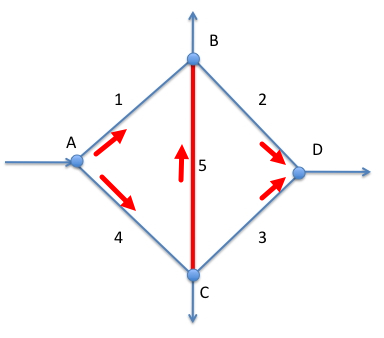
\includegraphics[width=5.1in]{wheatstone_bridge.jpg}
   \caption{Pipe network}
   \label{fig:wheatstone_bridge} 
\end{figure}

\begin{table}[h!]
%\footnotesize
   \centering
   \caption{Network properties for Figure \ref{fig:wheatstone_bridge}}
\begin{tabular}{lll}
\hline
Node&Demand (lps)&  Elevation(m) \\
\hline
A & -0.60 & 0.00 \\
B &  0.15   & 0.00 \\
C & 0.15 & 0.00 \\
D & 0.30 & 0.00 \\
\hline
Pipe& Length (m)&  Diameter (mm)\\
\hline
1 & 10,000 & 77.0 \\
2 & 10,000 & 77.0 \\
3 & 10,000 & 77.0 \\
4 & 10,000 & 77.0 \\
5 & 14,000 & 77.0 \\
\end{tabular}
\label{tab:wheatstone1}
\normalsize
\end{table}
\clearpage

%\item Referring to Figure \ref{fig:wheatstone_bridge}, the discharge in pipe 5 is closest to
%%standard answer set
%\begin{enumerate}[(A)]
%\item 0.00 cfs, from Node B to Node C  %Correct
%\item 0.15 cfs, from Node C to Node B
%\item 0.66 cfs, from Node C to Node B
%\item 0.66 cfs, from Node B to Node C
%\end{enumerate}


\item Critique the memorandum in Figure \ref{fig:memorandum}.  Mark directly on the figure -- you are to identify the grammar, spelling, punctuation and format errors and state the required corrections.

\begin{figure}[h!] %  figure placement: here, top, bottom, or page
\centering
   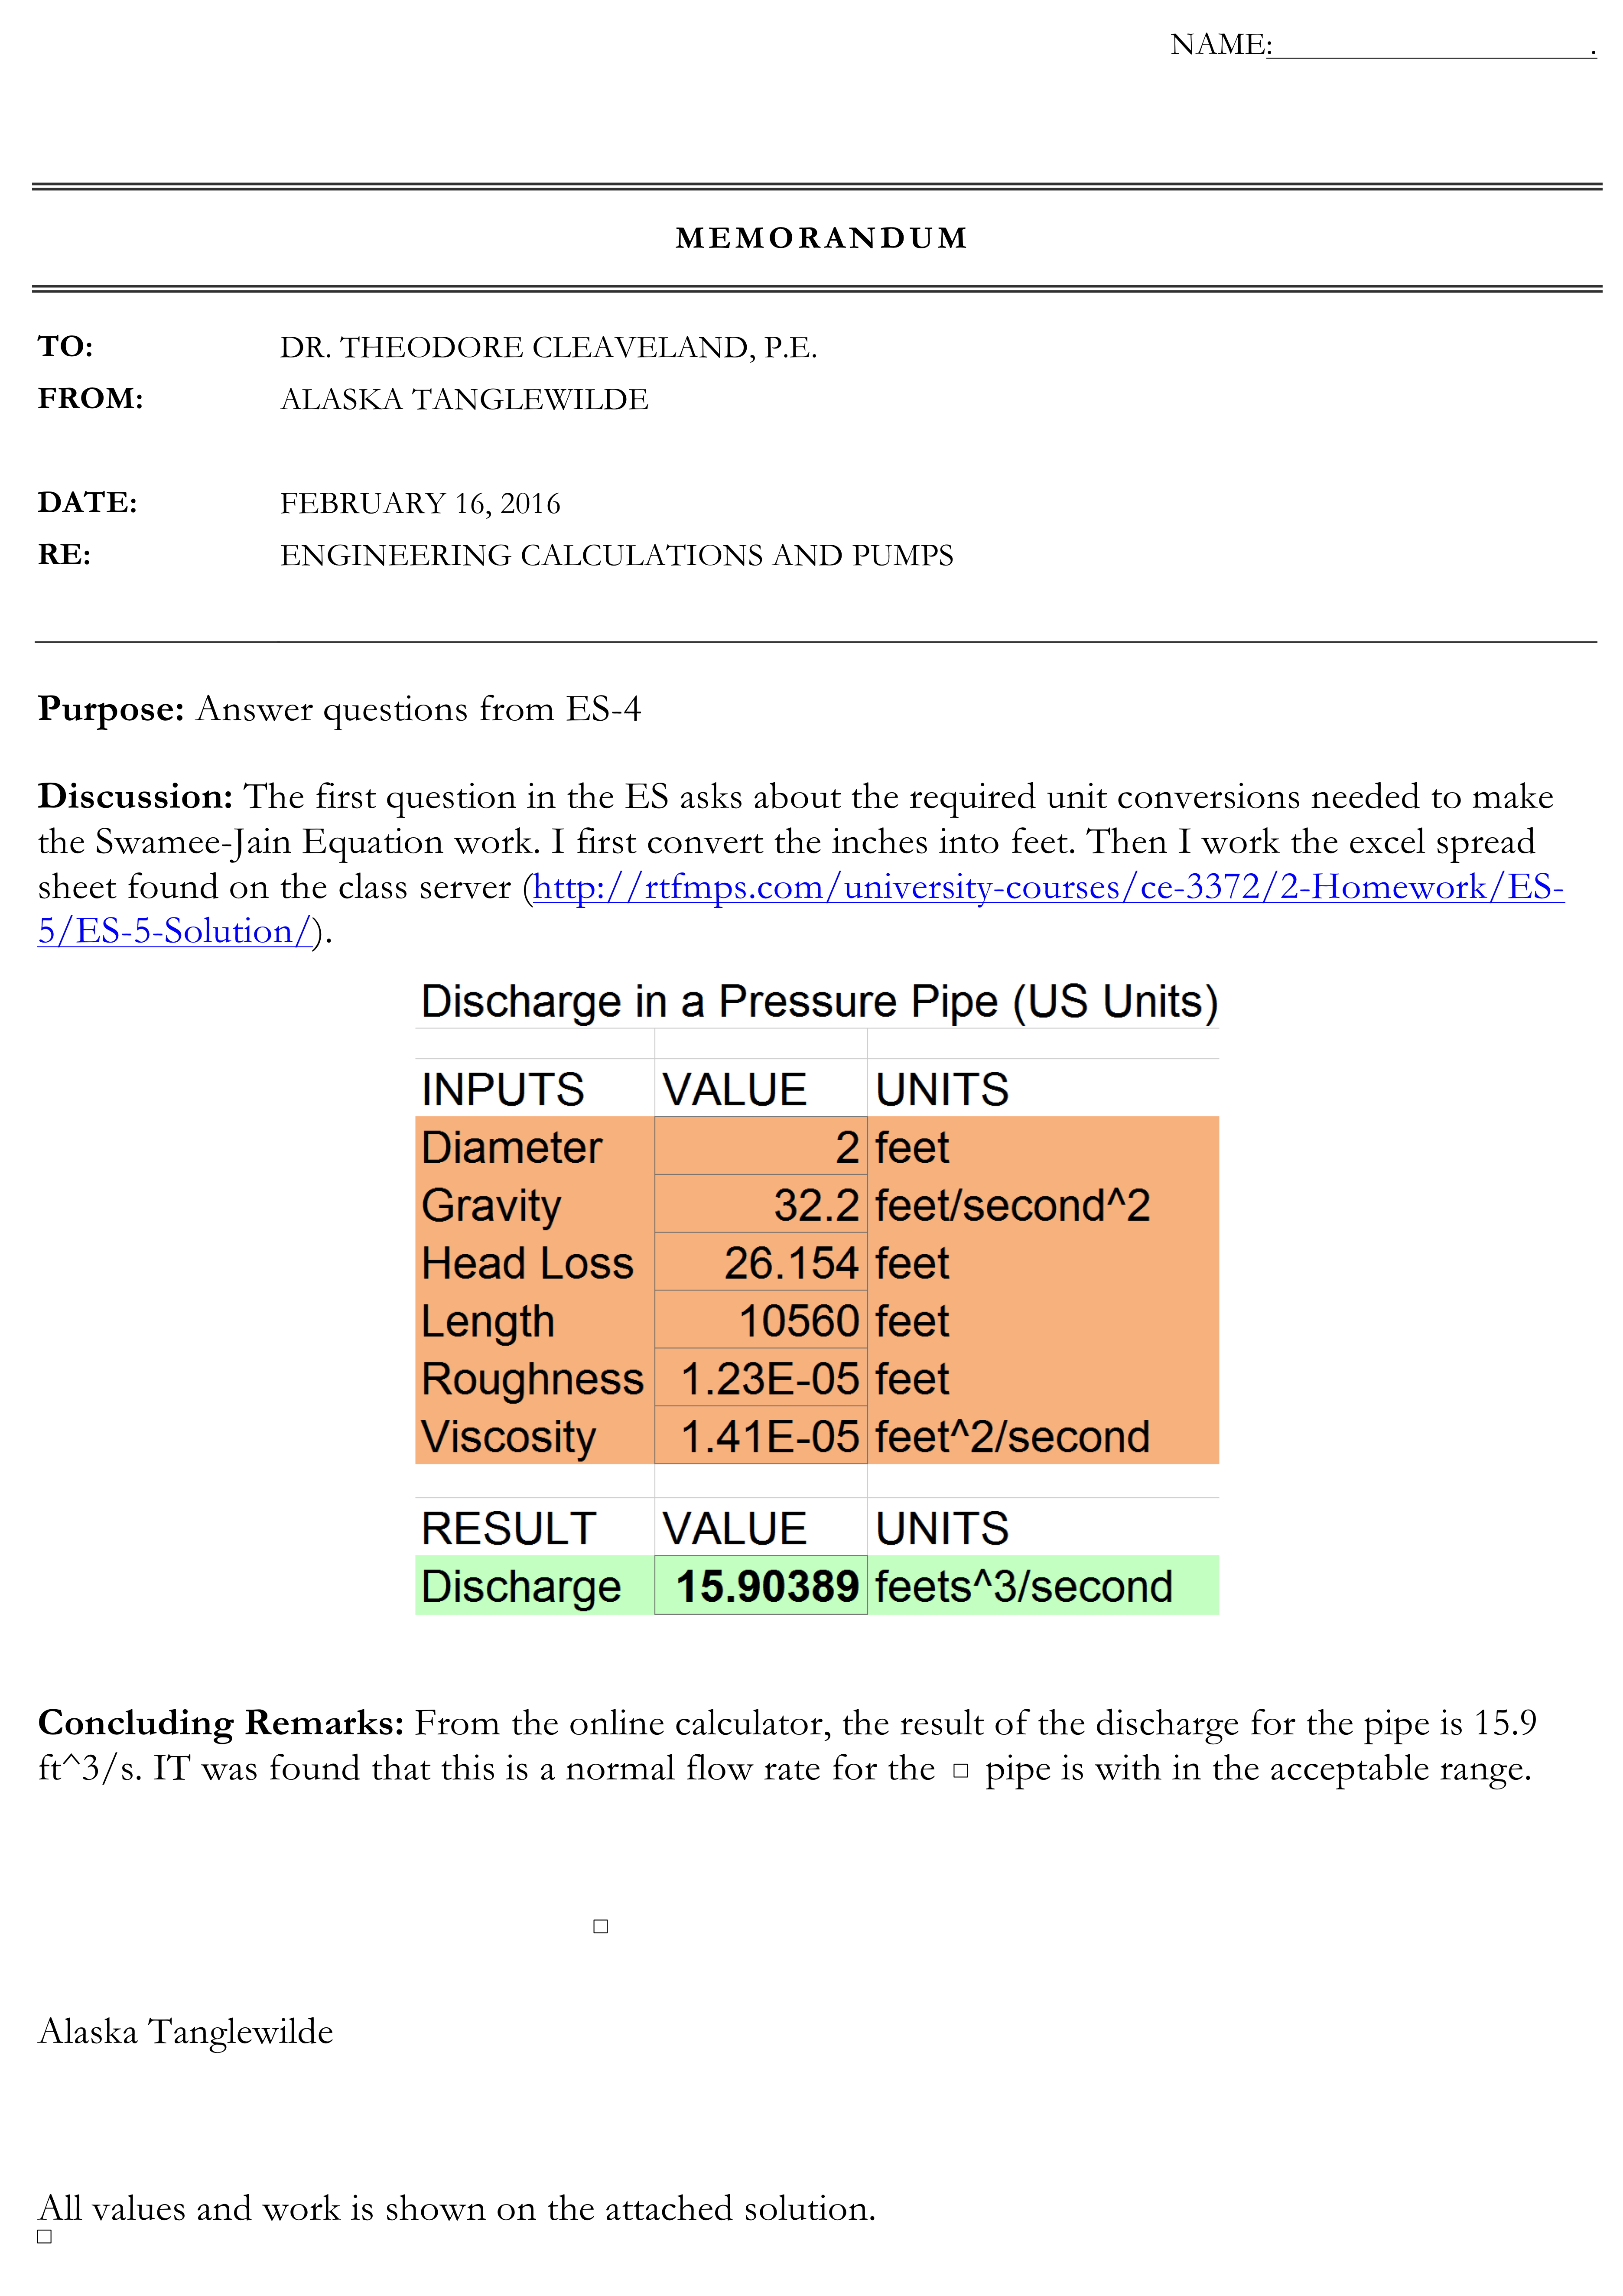
\includegraphics[height=7.3in]{Exam-1-Memo.jpg}
   \caption{Pipe network}
   \label{fig:memorandum} 
\end{figure}
